\chapter{Ideas and concepts}
\label{ch:Ideas-Concepts}
This chapter explains the different ideas and concepts used to realise the thesis. Some ideas were discovered during the research and were already introduced in the sections of related work (\ref{ch:Related-Work}) or were introduced in other approaches (\ref{sec:Other-Approaches}). Others were developed especially for this project and their application, as well as their advantages, will be proven in this work.
\newline
\newline
It is important to know that in the thesis, two distinct datasets are used to evaluate the application of the developed architecture in two domains. Due to that, many of the sections in this chapter are divided into two groups, one for the \fullref{sub:DCASE-Task-Dataset} and one for the music dataset (\ref{sub:Music-Dataset}).

\section{Data preprocessing}
\label{sec:Data-Preprocessing}
Data preprocessing is the process of processing the entire dataset before it is fed into the input pipeline (\ref{sec:Input-Pipeline}), either manually or automatically. Both datasets used in the project consist of audio files, which are grouped together by their corresponding label. Thus the structure of both datasets is very similar. For this thesis, it was decided that data preprocessing was not necessary for the \fullref{sub:DCASE-Task-Dataset}. However, for the music dataset (\ref{sub:Music-Dataset}), a minimal manual preprocessing is needed to improve the performance of the pipeline.
\newline
\newline
The \fullref{sub:DCASE-Task-Dataset} was already preprocessed by the organisers of the challenge. Which means that there are no audio files which contain multiple labels, are corrupted or invalid. The organisers of the challenge further split the sessions of recordings into 10s samples, which provides an easy and fast to use dataset. Therefore the preprocessing is neglected.
\newline
\newline
The music dataset (\ref{sub:Music-Dataset}) consists of different songs grouped by their respective genre. The audio samples in this dataset are given in the format of \texttt{.mp3} files, which is not that fast to process as for example \texttt{.wav} formatted audios. Therefore all of the \texttt{.mp3} audios were converted using \texttt{ffmpeg} to \texttt{.wav} files, with the simple script \ref{code:Convert-mp3-wav}.
\begin{code}[htbp]
\begin{minted}{bash}
for i in *.mp3; 
do ffmpeg -i "$i" "${i%.*}.wav";
done;
\end{minted}
\caption{Convert \texttt{.mp3} files to \texttt{.wav} files using \texttt{ffmpeg}}
\label{code:Convert-mp3-wav}
\end{code}
Further, the audios of the music dataset will be trimmed within the input pipeline (\ref{sec:Input-Pipeline}), because they should not contain any silence at the start or end of a song since this could lead to misclassified segments and clusters of silence, which should be omitted.

\section{Feature extraction}
\label{sec:Feature-Extraction}
Feature extraction, sometimes called feature representation, is the process of extracting the relevant features from the raw data; in this case, audio files. The extraction process is done within the input pipeline (\ref{sec:Input-Pipeline}). For both datasets, the same feature representations are used. Three different extractions are evaluated and are used as a hyperparameter which can be tuned to achieve the best possible performance. The optimal feature representation for the two datasets may be different since their characteristics are quite different. However, research has to show if that is the case.
\newline
\newline
The first approach is to use the audio files as they are, more precisely to use the raw waveform as input to the model. This is the most straightforward approach and as well the most lightweight to compute. It will be used to evaluate how good a model can be trained without any further feature extraction. The approach to use the raw waveform would be the simplest one to implement in a real-world application, because there is no complex computation needed, and can therefore as well be used on small devices, such as mobile phones or Raspberry Pis. However, when using the raw waveform of an audio segment, the preprocessing task of the input pipeline will get omitted, but the model gets a lot bigger since the input size is much larger than when using a feature representation. For example, when using the raw waveform of a 10s segment with the sample rate of 16'000, the input size gets 160'000, which is very large in comparison to the size when using a feature representation.
\newline
\newline
The second approach is to calculate the log-Mel spectrogram, which is outlined in subsection Mel spectrogram (\ref{sub:Mel-Spectrogram}), where the last step of calculating the \gls{DCT} is omitted. The process described was introduced to mimic the human hearing, but the last step, calculating the \gls{DCT}, was proposed because many machine learning models struggled with the highly correlated data, such as the log-Mel spectrogram, and thus a linear transformation (\gls{DCT}) was added to decorrelate the feature. Contemporary machine learning models such as \glspl{CNN} or \glspl{GRU} do not struggle with correlated data and perform even better when they can decorrelate the features themselves. Therefore this approach should give useful insight, weather the decorrelation can be trained and is still needed in present models. This approach is widely used in the audio domain because it is less computing extensive than calculating the \glspl{MFCC} and it can achieve almost the same, or an even better, accuracy as a model trained with the \glspl{MFCC} as their feature representation because it uses the same computations and additionally preserves more information.
\newline
\newline
The third and final approach is to calculate and use the \glspl{MFCC}, which is described in subsection Mel spectrogram (\ref{sub:Mel-Spectrogram}). This feature extraction method is used mainly in extensive audio applications, such as automatic speech and speaker recognition, where a lot of computing power is available. These features are mostly used because of their nature, that they represent sound like the human auditory system does, in a compact matter.
\newline
\newline
All of the features stated above are two-dimensional data, and therefore, standard image processing architectures can be adapted to audio processing. This adaption of image processing architectures to audio has successfully be shown in recent years of research \footcite{dai_acoustic_2016} \footcite{takahashi_deep_2016} \footcite{purwins_deep_2019} \footcite{lee_samplecnn_2018} \footcite{pons_timbre_2017}. 

\section{Triplet selection}
\label{sec:Triplet-Selection}
The triplet selection describes the process of selecting a neighbouring and opposite sample from a given anchor sample. The idea of triplet selection and the motivation behind it is described within section triplet loss (\ref{eq:Triplet-Loss}). The procedure is split into two parts, the selection of the neighbouring and opposite tile.
\newline
\newline
The straightforward way to triplet selection, as described in \ref{eq:Triplet-Loss} is to select the anchor and the neighbour to be part of the same label and to select the neighbour to have a different label than the other. However, this approach can not be used in an unsupervised learning technique because the data does not have any information about the underlying label. Due to that, a different, unsupervised approach to triplet selection has to be chosen.
\newline
\newline
For the triplet selection of the \fullref{sub:DCASE-Task-Dataset}, all of the 10s audio files have to be split into a specified \textit{sample length} (e.g. 1s, 2s) first. This results in different segments belonging to the same audio file, which are referred to as segments and denoted as $x$. The sample length specifies the length of all the segments. Therefore a triplet consists of three different segments $(x_a, x_n, x_o)$.
\newline
For the anchor tile $x_a$, a random segment is chosen. For the neighbouring tile $x_n$, a segment will be selected which belongs to the same audio file as the anchor, where the selection has to be done within a predefined range, \textit{neighbouring selection range} (e.g. 2s, 4s), of the anchor tile $x_a$. It is important to note, that it does not make any difference if the tile is being sampled from before or after the anchor segment. The segments $x_a$ and $x_n$ have to be distinct from each other and chosen within the specified \textit{neighbouring selection range}.
\newline
The opposite tile $x_o$ will be chosen at random from a different audio sample, where the selection of the segment is as well performed at random. The only constraint is that the opposite tile can not be chosen from the same audio file as the anchor and the neighbour.
\newline
\newline
For the music dataset (\ref{sub:Music-Dataset}), the triplet selection is made relatively similar to the one described in the paragraph above for the \fullref{sub:DCASE-Task-Dataset}. The only difference between the two methods is that for the music dataset, the audio files are of variable length. However, this does not make any difference in the selection process. The only difference between the two methods is that maybe the \textit{sample length} and \textit{neighbouring selection} range will need to be increased due to the increased audio file length, but this has to be shown in the experiments.

\section{Input pipeline}
\label{sec:Input-Pipeline}
\begin{figure}[htbp]
	\centering
	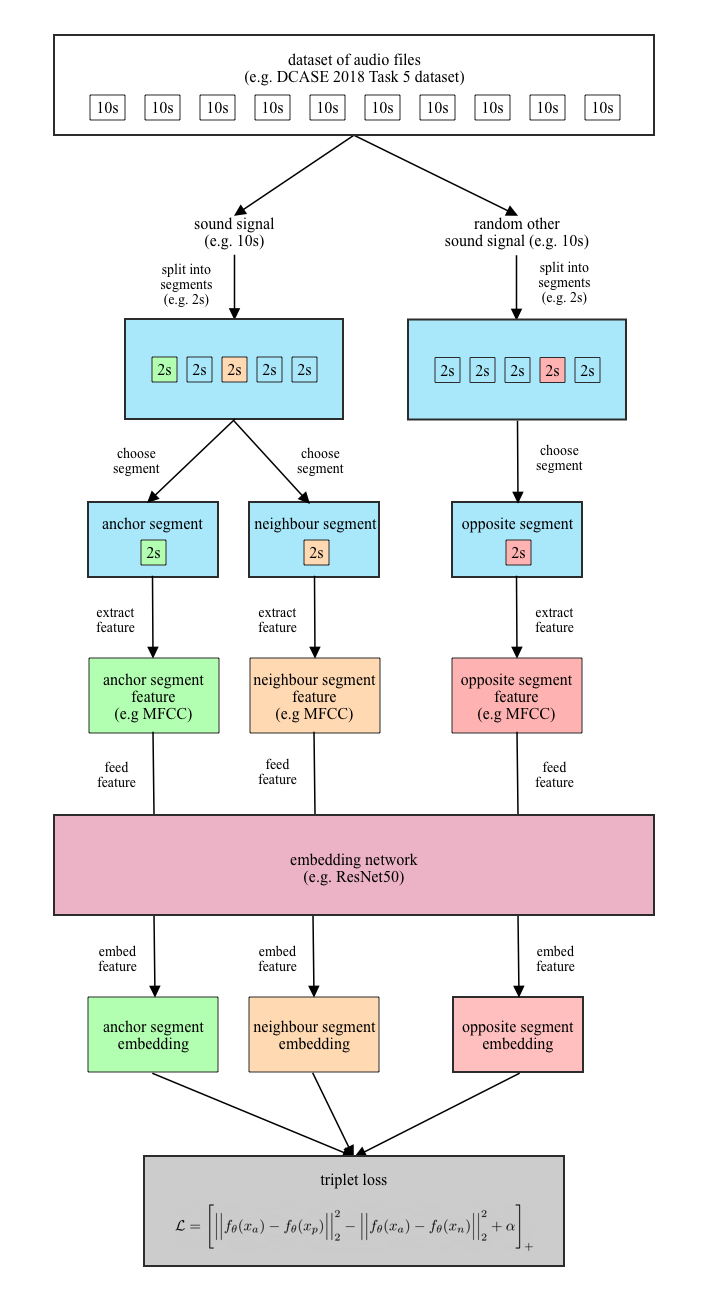
\includegraphics[scale=0.4]{img/Input_Pipeline_Visualisation.png}
	\caption{Visualisation of the input pipeline process}
	\label{fig:Input-Pipeline-Visualisation}
\end{figure}
\noindent
The input pipeline is responsible for creating the dataset, which will then be fed into the model by batches. For this project, the input pipeline is implemented using the TensorFlow \texttt{tf.data} API\footnotemark, along with a generator, which loops over the whole dataset and creates entries on the fly. The reason why a generator function is used, is that the entire dataset can not be loaded into memory, due to the large size of it. The entire process of the input pipeline is illustrated in figure \ref{fig:Input-Pipeline-Visualisation}.
\footnotetext{\url{https://www.tensorflow.org/api_docs/python/tf/data}}
\newline
\newline
The feature extraction (\ref{sec:Feature-Extraction}) and the triplet selection (\ref{sec:Triplet-Selection}) of the audio files is done on the fly within the input pipeline (\ref{sec:Input-Pipeline}). The advantage of this method is that the pipeline can be adapted fairly quick for other datasets since the only input the pipeline requires is the raw waveform of an audio signal of any kind. 
\newline
\newline
The first step of the input pipeline is to loop over the corresponding generator function of the specified dataset, which loops over the entire dataset and returns the current sample of the dataset. For each one of the returned samples, a triplet, consisting of an anchor, neighbour and an opposite audio segment, is created by using the datasets method to perform the selection. The triplet, which will be returned from the dataset consists of indices of the audio and segment for each one of the three segments. Then the input pipeline uses these indices to extract the corresponding audio segment out of the dataset and yields them back to the \texttt{tf.data.Dataset}. It is important to note that all the operations listed after this paragraph are done on the whole batch.
\newline
\newline
After the dataset gets an entire batch of audio segments, the feature extraction will be performed. The feature extraction is implemented using the vectorised \texttt{.map} function of the class \texttt{tf.data.Dataset}\footnotemark. The \texttt{.map} function applies a given function to each element within the dataset, which in the case of this thesis will be used to extract the features from the audio. Hence a \flqq feature extractor\frqq \ has to be provided to the input pipeline, which will extract a certain feature from the audio as stated in \ref{sec:Feature-Extraction}. If no extractor is passed to the pipeline, the raw waveform of the signal is used. 
\footnotetext{\url{https://www.tensorflow.org/api_docs/python/tf/data/Dataset}}
\newline
\newline
After the extraction, the dataset is shuffled and returned to the training process. In the training loop, the dataset can now be iterated over, which yields back a batch of triplets, consisting of the extracted audio segment. This batch can then be used to train the model. The dataset is therefore similar to a Python iterator.
\newline
\newline
The advantages of this method are that this creates the dataset dynamically, because the dataset only contains the current batch along with some prefetched entries, which are entries from the next batch so that the \gls{GPU} can be fully utilised.

\section{Models}
\label{sec:Models}
This section describes the overall architecture of the models used in the thesis. The idea of the thesis is to evaluate different kinds of architectures and compare their results to find the optimal model for the thesis.
\newline
\newline
The first architecture, which will be evaluated are \glspl{CNN} (\ref{sub:Convolutional-Neural-Network}). They are used in a lot of audio applications because of their simplicity and robustness. A considerable amount of research in the past couple of years has shown the overall success of these models. Therefore it makes sense to evaluate these type of models extensively. Subsection \ref{sub:ResNet} describes a state-of-the-art \gls{CNN} architecture, which will be mainly used throughout the thesis.
\newline
\newline
Another widely used model architecture is the \gls{RNN}, where \glspl{GRU} (\ref{sub:Gated-Recurrent-Unit}) is one of the most prominent implementations. Their application primarily lies in the text-domain. However, in recent years they have shown their success within the audio domain, mainly because of the sequential nature of the audio signal.
\newline
\newline
The most prominent approach in audio research is the combination of \glspl{CNN} and \glspl{RNN}. The architecture consists of multiple convolution layers, and a single or multiple recurrent layers. The idea of these models is that they first reduce the input data to a specific lower-dimensional representation and then use recurrent models to make use of the sequential nature of the audio. Therefore the best ideas of both architectures are used within these \glspl{CRNN}.
\newline
\newline
For the implementation and the experiments, \glspl{CNN} should be mainly used, and if there is time, to evaluate and implement state-of-the-art \gls{RNN} and \gls{CRNN} models.

\subsection{ResNet}
\label{sub:ResNet}
\Gls{ResNet} is a state-of-the-art \gls{CNN} architecture, which was introduced in 2015 (\cite{he_deep_2015}), and was the winner of ImageNet Visual Recognition Challenge 2015. The problem \gls{ResNet} solves is the degradation problem, which has been observed when deeper networks start converging. The problem states, that with the network depth increasing, accuracy gets saturated and then degrades rapidly. Therefore, using deeper networks is degrading the performance of the model. \cite{he_deep_2015} tries to solve this problem using deep residual learning framework. The core idea introduced are so-called \flqq identity shortcut connection\frqq \ that skip one or more layers, as shown in figure \ref{fig:ResNet-Residual-Block}. Typical \gls{ResNet} models are implemented with double- or triple- layer skips that contain non-linearities (ReLU) and batch normalization in between, as shown in figure \ref{fig:ResNet-Skip-Layers}. The whole architecture is a stack of residual blocks with appropriate stride and pooling. These residual networks are easier to optimise and can gain accuracy from considerably increased depth. They have shown their applicability in much research in recent years and should, therefore, be used as the main model architecture throughout this thesis.
\begin{figure}[htb]
\centering
\begin{subfigure}{.5\linewidth}
  \centering
  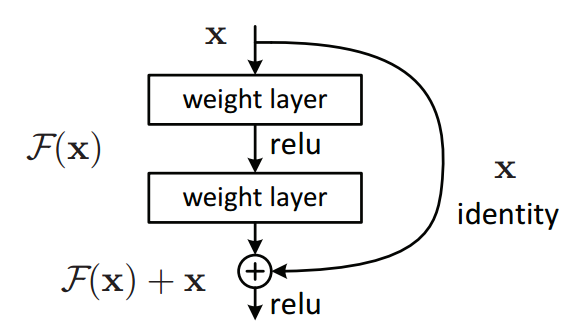
\includegraphics[width=\linewidth]{img/ResNet_SkipConnections.png}
  \caption{Residual block}
  \label{fig:ResNet-Residual-Block}
\end{subfigure}%
\begin{subfigure}{.5\linewidth}
  \centering
  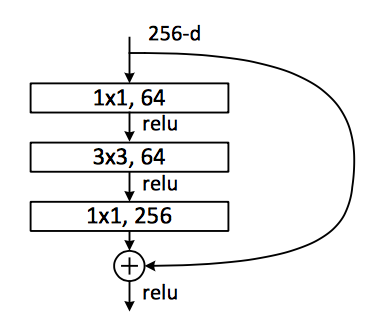
\includegraphics[width=.75\linewidth]{img/ResNet_Stacks.png}
  \caption{Triple layer skip connection}
  \label{fig:ResNet-Skip-Layers}
\end{subfigure}
\caption[ResNet visualisations]{ResNet visualisations\footnotemark}
\label{fig:ResNet-Visualisations}
\end{figure}
\footnotetext{\fullcite{he_deep_2015}}

\section{Application to music}
\label{sec:Application-Music}
All of the concepts mentioned above are designed to work with both datasets. Thus the application to music is described in each of the sections above separately. But to summarise, to adapt the model from the noise detection dataset to the music dataset, the same architecture will be used. This includes using the same triplet selection process. However, almost inevitably, the segments will need to be increased. Then to use the same input pipeline, with the same feature representation. This results in almost the same architecture as for the \gls{DCASE} dataset, with a few exceptions.

\section{Metrics}
\label{sec:Metrics}
Meaningful metrics need to be used to evaluate and compare the performance of machine learning models. In supervised machine learning, most of the metrics focus on how well the model predicts the actual value from the input, but in the unsupervised setting, finding meaningful metrics is a lot harder. Hence the metrics for the embedding model and the classifier are quite different because the embedding architecture is unsupervised while the classifier is supervised. Therefore this section is split into two parts, metrics for the embedding space (\ref{sub:Metrics-Embedding-Space}) and metrics for the classifier (\ref{sub:Metrics-Classifier}), which both aim to give valuable insights into the performance. All of the mentioned metrics below are monitored using the Tensorboard visualisation toolkit\footnote{\url{https://www.tensorflow.org/tensorboard}}.

\subsection{Embedding space}
\label{sub:Metrics-Embedding-Space}
As mentioned before, it is not easy to find meaningful metrics for the embedding space because of its unsupervised nature. However, since the thesis focuses on the application of triplet loss in the unsupervised setting, one of the most straight forward metrics to use is to monitor the triplet loss value, which gives insight if the model is training and learning a representation over time. Thus this value should be minimized over time. The triplet loss value, which will be monitored, results out of the equation \ref{eq:Triplet-Loss}. Since the idea of triplet loss is to minimize the distance between the anchor and the positive sample and to maximize the distance between the anchor and the negative sample, it makes sense to monitor them. Both values are already computed when computing the triplet loss and only have to be monitored. As a distance measure between the embeddings, the squared euclidean distance, given by equation \ref{eq:Euclidean-Distance}, is used. Monitoring these distances, give valuable insights if the model is capable of satisfying the triplet loss constraint or not. All of these three metrics are monitored both on the training and evaluation dataset.
\newline
\newline
The embedding space can further be thought of as a clustering task, where the goal is to cluster similar samples in the near-by region. Since the evaluation set contains the ground truth of each sample, most clustering metrics can be used to monitor the progress of the embedding space. 
\newline
\newline
One of the most straightforward metrics to use for evaluation and comparison of the resulting embedding spaces is the distances between the clusters. They can be computed by calculating the distance from each centroid of a cluster to every other. The metric gives an insight into how distant the clusters of each label are. It can be displayed in two different ways, as different graphs and as a distance matrix in the form of an image. Such a representation in the form of an image is shown in figure \ref{fig:Distance-Matrix}. However, it is important to say that this metric is very vulnerable for outliers, which means that the centroid can vary very broadly if one of the clusters contains many outliers.
\newline
\newline
Further, a popular clustering metric called the silhouette coefficient, is used, where a higher score relates to a model with better-defined clusters. The score is bounded between $-1$ for incorrect clustering and $+1$ for highly dense clustering. Scores around zero indicate overlapping clusters. The score is higher when clusters are dense and well separated, which relates to a standard concept of a cluster. The silhouette coefficient is defined for each sample and is composed of two scores:
\begin{itemize}
\setlength\itemsep{0em}
    \item $a$: The mean distance between a sample and all other points in the same class
    \item $b$: The mean distance between a sample and all other points in the next nearest cluster
\end{itemize}
The silhouette coefficient $s$ for a single sample is then given by equation \ref{eq:Silhouette-Coefficient}. For a set of samples, the silhouette coefficient is given as the mean of the silhouette coefficient for each sample.
\myequations{Silhouette coefficient for a single sample}
\begin{equation}
    \centering
    \begin{gathered}
        s = \frac{b - a}{max(a, b)}
    \end{gathered}
    \label{eq:Silhouette-Coefficient}
\end{equation}
Both of the metrics above are only computed on the evaluation dataset, since monitoring it on the training set would not provide more insight.
\begin{figure}[htbp]
	\centering
	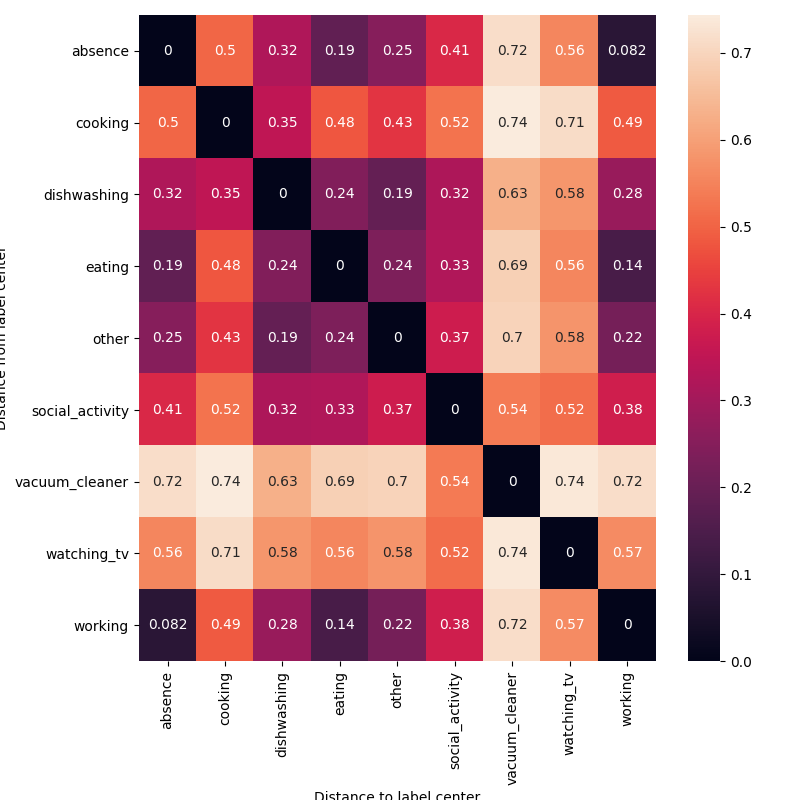
\includegraphics[scale=0.3]{img/Distance_Metric.png}
	\caption{Distance matrix from each centroid to every other}
	\label{fig:Distance-Matrix}
\end{figure}

\subsection{Classifier}
\label{sub:Metrics-Classifier}
For the classifier, standard supervised metrics are monitored, such as loss and accuracy. The loss function used to train the model is the sparse categorical cross-entropy loss. Therefore this loss function will be monitored to show if the model minimises this function over time. As an accuracy metric, the sparse categorical accuracy is monitored to show how well the classifier predicts the inputs.
\newline
\newline
The usage of the accuracy does not work well with highly unbalanced datasets such as the \fullref{sub:DCASE-Task-Dataset}. Therefore another metric needs to be used, which works well with this kind of dataset. The organisers of the \gls{DCASE} task 5 challenge used the macro-averaged F1 score to evaluate the models' performance. This score satisfies the constraint of working well with unbalanced data and is therefore used to monitor the accuracy of the classifier as well. Furthermore, it is used to compare the results accomplished in the thesis, to the results by other models submitted in the challenge. The F1 score is given by equation \ref{eq:F1-Score} and to get the macro-averaged F1 score, the metric has to be calculated for each label, and then the unweighted mean is taken.
\myequations{F1 score}
\begin{equation}
    \centering
    \begin{gathered}
        \text{F1} = 2 \cdot \frac{\text{precision} \cdot \text{recall}}{\text{precision} + \text{recall}} \\
        \text{precision} = \frac{\text{TP}}{\text{TP} + \text{FP}} \\
        \text{recall} = \frac{\text{TP}}{\text{TP} + \text{FN}} \\
    \end{gathered}
    \label{eq:F1-Score}
\end{equation}
where:
\begin{conditions*}
    \text{TP} & true positive \\   
    \text{TN} & true negative \\ 
    \text{FP} & false positive \\ 
    \text{FN} & false negative \\ 
\end{conditions*}
\noindent
All of the metrics for the classifier are both monitored for the training as well as the evaluation dataset.